\section{Introduction}
\label{sec:introduction}

\begin{figure}[t]
    %\vspace*{-2px}
    
    \hspace*{-0.25cm}
    \begin{minipage}[t]{0.5\textwidth}
        \vspace*{-10px}
        \centering
        \begin{minipage}{0.495\textwidth}
        	\begin{tcolorbox}[
        		left=0pt,
        		right=0pt,
        		top=0pt,
        		bottom=0pt,
        		colback=white,
        		colframe=gray!10!white,
        		width=1\textwidth, 
        		enlarge left by=0mm,
        		boxsep=5pt,
        		arc=0pt,outer arc=0pt,
        		boxrule=1pt,
        		]
        		
        		\centering
        		\small\textbf{Adversarial Training (\AdvTrain):}
                \vspace*{-1px}
        	\end{tcolorbox}
            \begin{tcolorbox}[
                left=0pt,
                right=0pt,
                top=0pt,
                bottom=0pt,
                colback=white,
                colframe=gray!10!white,
                width=1\textwidth, 
                enlarge left by=0mm,
                boxsep=5pt,
                arc=0pt,outer arc=0pt,
                boxrule=1pt,
                ]
                
                \vspace*{-4px}
                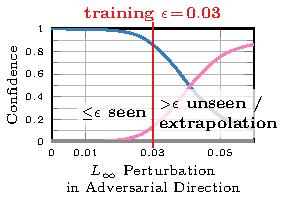
\includegraphics[width=3.8cm]{fig_intro_advtrain_1_adversarial}
                \vskip -2px
                
                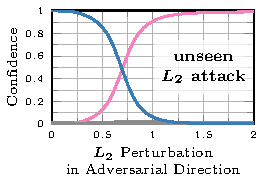
\includegraphics[width=3.5cm]{fig_intro_advtrain_3_l2_adversarial}
                \vspace*{-6px}
            \end{tcolorbox}
        \end{minipage}
        \hfill
        \begin{minipage}{0.495\textwidth}
        	\begin{tcolorbox}[
        		left=0pt,
        		right=0pt,
        		top=0pt,
        		bottom=0pt,
        		colback=gray!12!white,
        		colframe=gray!12!white,
        		width=1\textwidth, 
        		enlarge left by=0mm,
        		boxsep=5pt,
        		arc=0pt,outer arc=0pt,
        		boxrule=1pt,
        		]
        		
        		\centering
        		\small\textbf{Ours (CCAT):}
                \vspace*{-1px}
        	\end{tcolorbox}
            \begin{tcolorbox}[
                left=0pt,
                right=0pt,
                top=0pt,
                bottom=0pt,
                colback=gray!12!white,
                colframe=gray!12!white,
                width=1\textwidth, 
                enlarge left by=0mm,
                boxsep=5pt,
                arc=0pt,outer arc=0pt,
                boxrule=1pt,
                ]
                
                \vspace*{-4px}
                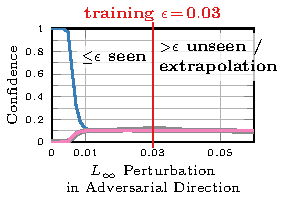
\includegraphics[width=3.8cm]{fig_intro_ours10_1_adversarial}
                \vskip -2px
                
                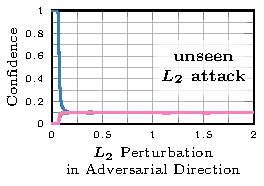
\includegraphics[width=3.5cm]{fig_intro_ours10_3_l2_adversarial}
                \vspace*{-6px}
            \end{tcolorbox}
        \end{minipage}
    
        \begin{tcolorbox}[
            left=0pt,
            right=0pt,
            top=0pt,
            bottom=0pt,
            colback=white,
            colframe=gray!10!white,
            width=1\textwidth, 
            enlarge left by=0mm,
            boxsep=5pt,
            arc=0pt,outer arc=0pt,
            boxrule=1pt,
            ]
            \centering
            \scriptsize
            
            \textcolor{colorbrewer2}{{\rule[2pt]{10pt}{1pt} (Correct) Predicted Class}}\xspace\xspace\xspace \textcolor{colorbrewer8}{{\rule[2pt]{10pt}{1pt} Adversarial Class}}\xspace\xspace\xspace \textcolor{colorbrewer9}{{\rule[2pt]{10pt}{1pt} Other Classes}}
        \end{tcolorbox}
    \end{minipage}
    \vskip -2px
    
    \caption{
    \textbf{Adversarial Training (\AdvTrain) versus our \ConfTrain.} We plot the confidence in the 
    direction of an adversarial example. AT enforces high
    confidence predictions for the correct class on the $L_\infty$-ball of radius $\epsilon$ (\emph{``seen''}
    attack during training, top left). As AT
    enforces no particular bias beyond the $\epsilon$-ball, adversarial examples can be found right beyond this ball. In contrast \ConfTrain enforces a decaying confidence in the correct class up to uniform confidence within the $\epsilon$-ball (top right). Thus, \ConfTrain biases the model to extrapolate uniform confidence beyond
    the $\epsilon$-ball. This behavior also extends to \emph{``unseen''} attacks during training, \eg, $L_2$ attacks (bottom), such that adversarial examples can be
    rejected via confidence-thresholding.
    }
    \label{fig:introduction}
    \vspace*{-2px}
\end{figure}

Deep networks were shown to be susceptible to adversarial examples \cite{SzegedyICLR2014}: adversarially perturbed examples that cause mis-classification while being nearly ``imperceptible'', \ie, close to the original example. Here, ``closeness'' is commonly enforced by constraining the $L_p$ norm of the perturbation, referred to as threat model. Since then, numerous defenses against adversarial examples have been proposed. However, many were unable to keep up with more advanced attacks \cite{AthalyeICML2018b,AthalyeARXIV2018b}. Moreover, most defenses are tailored to only one specific threat model.

Adversarial training \citep{GoodfellowICLR2015,MadryICLR2018}, \ie, training on adversarial examples, can be regarded as state-of-the-art. However, following \figref{fig:introduction}, adversarial training is known to ``overfit'' to the threat model \emph{``seen''} during training, \eg, $L_\infty$ adversarial examples.
Thus, robustness does not extrapolate to larger $L_\infty$ perturbations, \cf \figref{fig:introduction} (top left), or generalize to \emph{``unseen''} attacks, \cf \figref{fig:introduction} (bottom left), \eg, other $L_p$ threat models \citep{SharmaICLRWORK2018,TramerNIPS2019,LiARXIV2019,KangARXIV2019,MainiICML2020}.
We hypothesize this to be a result of enforcing high-confidence predictions on adversarial examples. However, high-confidence predictions are difficult to extrapolate beyond the adversarial examples seen during training. Moreover, it is not meaningful to extrapolate high-confidence predictions to arbitrary regions.
Finally, adversarial training often hurts accuracy, resulting in a robustness-accuracy trade-off \citep{TsiprasICLR2019,StutzCVPR2019,RaghunathanARXIV2019,ZhangICML2019}.

\textbf{Contributions:}
%
We propose \textbf{confidence-calibrated adversarial training (\ConfTrain)} which trains the network to predict a convex combination of uniform and (correct) one-hot distribution on adversarial examples that becomes more uniform as the distance to the attacked example increases. This is illustrated in \figref{fig:introduction}. Thus, \ConfTrain implicitly biases the network to predict a uniform distribution beyond the threat model \emph{seen} during training, \cf \figref{fig:introduction} (top right). Robustness is obtained by rejecting low-confidence (adversarial) examples through confidence-thresholding. As a result, having seen \emph{only} $L_\infty$ adversarial examples during training, \ConfTrain improves robustness against previously \emph{unseen} attacks, \cf \figref{fig:introduction} (bottom right), \eg, $L_2$, $L_1$ and $L_0$ adversarial examples or larger $L_\infty$ perturbations. Furthermore, robustness extends to adversarial frames \cite{ZajaxAAAIWORK2019}, distal adversarial examples \cite{HeinCVPR2019}, corrupted examples (\eg, noise, blur, transforms \etc) and accuracy of normal training is preserved better than with adversarial training.

For thorough evaluation, following best practices \cite{CarliniARXIV2019}, we adapt several state-of-the-art white- and black-box attacks \cite{MadryICLR2018,IlyasICML2018,AndriushchenkoARXIV2019,NarodytskaCVPRWORK2017,KhouryARXIV2018} to \ConfTrain by explicitly maximizing confidence and improving optimization through a backtracking scheme. In total, we consider $7$ different attacks for each threat model (\ie, $L_p$ for $p \in \{\infty, 2, 1, 0\}$), allowing up to $50$ random restarts and $5000$ iterations each. We report worst-case robust test error, extended to our confidence-thresholded setting, across \emph{all} attacks and restarts, on a \emph{per test example} basis. We demonstrate improved robustness against unseen attacks compared to standard adversarial training \cite{MadryICLR2018}, TRADES \cite{ZhangICML2019}, adversarial training using multiple threat models \cite{MainiICML2020} and two detection methods \cite{MaICLR2018,LeeNIPS2018}, while training \emph{only} on $L_\infty$ adversarial examples.

We make our code (training and evaluation) and pre-trained models publicly available at \href{http://davidstutz.de/ccat}{davidstutz.de/ccat}.